\chapter{基于PW对的两阶段调度模型}

\setcounter{equation}{0}

一次生产处理或清洁处理对应一个加工周期，其中生产周期指按产品配方执行工艺处理的周期。清洁处理仅由辅助晶圆占位，其阈值至少为2。

模型输入包括动作时长、资源容量、驻留上限、清洁阈值和辅助晶圆数量，输出为具体晶圆的资源指派及动作起止时刻。
表~\ref{tab:symbol-cn-a}定义输入常量与集合，表~\ref{tab:symbol-cn-b}定义主要决策变量及辅助变量，其余符号在正文首次使用处定义。
所有时刻和时长的单位均为秒，数量的单位为片、对或周期。

\begin{table}[!htbp]
\centering\small
\caption{批次任务调度的输入参数与集合配置}
\label{tab:symbol-cn-a}
\renewcommand{\arraystretch}{1.03}
\setlength{\tabcolsep}{4pt}
\begin{adjustbox}{max width=\linewidth,max totalheight=0.92\textheight}
\begin{tabular}{@{}>{\raggedright\arraybackslash}p{0.26\textwidth}p{\dimexpr0.74\textwidth-8pt\relax}@{}}
\toprule
符号 & 定义与取值\\\midrule
$\mathcal J,\mathrm{Pjob}_j$ & $\mathcal J=\{1,\ldots,J\}$是批次任务集合；$\mathrm{Pjob}_j$是任务$j$的产品晶圆集合。\\
$\mathcal L_j,\ell_{jk}$ & $\mathcal L_j$是任务$j$实际晶圆编号的升序表，$\ell_{jk}$是其第$k$片晶圆的来源LP编号。\\
$N_{j\ell},N_j,N_\zeta,N_\psi,N$ & 分别表示任务$j$在LP $\ell$的产品数、任务$j$的产品总数、两种生产配方的产品数及全批产品总数。\\
$m_j,\mathcal M,\mathcal C_j$ & $\mathcal M=\{\zeta,\psi,\mathrm{cl}\}$是加工类型集合，三种标签依次表示$4\times1$、$2\times2$与清洁；$m_j$是任务$j$的加工模式类型。$\mathcal C=\{\mathrm{CH2},\mathrm{CH3}\}$是腔室集合，$\mathcal C_j\subseteq\mathcal C$是任务$j$允许访问的非空腔室集合。\\
$\mathcal P,\mathcal Q_c,\mathcal I$ & $\mathcal P=\{1,\ldots,P_{\max}\}$是PW对集合；$\mathcal Q_c=\{1,\ldots,Q_{\max}\}$是腔室$c$的周期集合；$\mathcal I=\mathcal P\times\{0,1\}$是晶圆路线任务集合。\\
$T,J_{\max},P_{\max},Q_{\max}$ & 依次表示全设备生产周期数上界、清洁次数上界、PW对容量和每腔候选周期容量。\\
$\mathcal S,\sigma$ & $\mathcal S=\{A,V\}$是来源区域集合，元素分别是大气区、真空区；$\sigma$表示来源配置，单源取0、双源取1。\\
$\mathcal O,\mathcal O^{\rm occ}$ & $\mathcal O$是候选物理动作集合，$\mathcal O^{\rm occ}$是候选资源占用区间集合，由路线与周期模板生成。\\
$\mathcal R,K_\rho,\mathcal D$ & $\mathcal R$是资源集合，$K_\rho$是资源$\rho$的容量：ATR承2片、VTR承4片，AL容量1片，上/下LL各2槽，腔室4工位，$\mathcal D=\{1,\ldots,D\}$是辅助晶圆集合，默认$D=8$，两个腔时存储容量为10片。\\
$d_m\ (d_\zeta,d_\psi,d_{\mathrm{cl}})$ & 表示类型$m$的加工持续时间，默认$(d_\zeta,d_\psi,d_{\mathrm{cl}})=(180,90,500)$~s；$2\times2$产品需相邻两次加工处理。\\
$d_o^{\rm ATR},d_o^{\rm VTR},r_c$ & 分别表示ATR取放时长、VTR取放时长和腔室$c$半周旋转时长，默认分别为4、1、2~s。\\
$t_{\rm ATR},t_{\rm VTR},t_{\rm empty}$ & 分别表示ATR交换时长、VTR交换时长和ATR从LL移动LP的时长，默认分别为3、2、6~s。\\
$t_{\rm AL},t_{\rm pump},t_{\rm vent}$ & 分别表示产品对准、上LL抽气及下LL放气时长，默认分别为20、30、25~s；辅助片不执行AL对准。\\
$t_{\rm U}^{\rm reset},t_{\rm L}^{\rm reset}$ & 分别表示上/下LL槽位复位时长，默认分别为30、25~s，从另一侧取片结束后开始计。\\
$d_o,\delta_{oo'},\delta^\rho_{oo'}$ & 分别表示动作$o$的持续时间、$o$结束至后续动作$o'$开始的时间间隔、资源$\rho$从$o$至$o'$的换位或复位间隔。\\
$H$ & 表示清洁阈值，$H\ge2$，默认$H=3$；累计1至$H-1$次可提前清洁，达到$H$必须清洁。\\
$\overline R_{i\rho}$ & 表示路线任务$i$在资源$\rho$的驻留上限；模块按放片结束至取片开始计，工艺腔另扣除必要处理时长；机械手按取片开始至放片结束计。\\
$B,M$ & 分别表示整个加工排程的时间上界和加上必要间隔的约束松弛量；默认$B=10000$~s，装载锁复位须在时域内完成；后者取$M=B+\max\{\delta_{oo'},\delta^\rho_{oo'},r_c\}$。\\
$\lambda_1,\lambda_2,\lambda_3$ & 依次是总等待、最大单项等待与节拍变化的非负权重，默认$(\lambda_1,\lambda_2,\lambda_3)=(1,10,25)$。\\
$\varepsilon_C$ & 产品完工上界容差，默认$10^{-6}$~s。\\
\bottomrule
\end{tabular}
\end{adjustbox}
\end{table}

\begin{table}[!htbp]
\centering\small
\caption{批次任务调度的关键决策变量}
\label{tab:symbol-cn-b}
\renewcommand{\arraystretch}{1.05}
\setlength{\tabcolsep}{4pt}
\begin{adjustbox}{max width=\linewidth}
\begin{tabular}{@{}>{\raggedright\arraybackslash}p{0.23\textwidth}p{0.18\textwidth}p{0.55\textwidth}@{}}
\toprule
符号 & 类型 & 定义与取值含义\\\midrule
$x_{j\ell pr}$ & 二元决策变量 & PW对$p$的位置$r$是否使用任务$j$在LP $\ell$的一片产品，$N_{j\ell}>0$时建立。\\
$v_p,\mu_{pm},z_{pc}$ & 二元决策变量 & 分别表示PW对$p$是否启用，是否采用加工类型$m$，是否分配至腔室$c$。\\
$X_{pcq},K_{cqm},f_{pcq}$ & 二元决策变量 & 分别表示PW对$p$是否占用腔室$c$的周期$q$，周期$q$是否采用类型$m$，对$p$在腔室$c$的周期$q$是否位于可访问侧。\\
$g_{pr\tau}$ & 二元决策变量 & 表示对内位置$(p,r)$是否借用辅助晶圆$\tau\in\mathcal D$。\\
$h_{ou},y^\rho_{oo'},\gamma_{pa}$ & 二元决策变量 & 分别表示动作$o$是否选择物理单元$u$，在同一资源$\rho$时$o$是否先于$o'$，对$p$的两片晶圆在取放段$a$同步搬运，标签$\mathrm{pick}$表示源LP端取片。\\
$s_o,S_{cq}$ & 非负实数决策变量 & 分别表示物理动作$o$和腔室$c$的周期$q$的开始时刻。\\
$e_o,b_o$ & 辅助变量 & $e_o$表示动作$o$的结束时刻；$b_o$是二元辅助变量，表示动作$o$是否启用。\\
$\theta_{j\ell}$ & 非负实数辅助变量 & 任务$j$在相邻非空LP之间切换取片的时间分界点。\\
$n_{cq}$ & 非负整数辅助变量 & 腔室$c$第$q$个周期结束后，自上次清洁以来累计完成的生产周期数，范围为$0,\ldots,H$。\\
$F_p,F_p^\psi,X^P_{pcq}$ & 二元辅助变量 & 分别表示对$p$是否含产品，是否含$2\times2$产品，是否参加腔室$c$的周期$q$。\\
$\beta_{pr},d_{pr}$ & 二元辅助变量 & $\beta_{pr},d_{pr}$ 分别表示对内位置$(p,r)$是否安排产品、是否借用辅助片。\\
$\chi_{iA},\chi_{iV}$ & 二元辅助变量 & $\chi_{iA},\chi_{iV}$分别表示路线任务$i$是否由大气区、真空区供给。\\
$C_{\max}$ & 非负实数决策变量 & 产品返回原LP时刻的上界。\\
$L_{\max},v_{cq}$ & 非负实数辅助变量 & $L_{\max}$为所有等待项的上界；$v_{cq}$为以$(c,q)$为中心的相邻周期开始间隔变化量的绝对值上界。\\
\bottomrule
\end{tabular}
\end{adjustbox}
\end{table}

\section{批次任务与产品晶圆编码}
\label{sec:model-encoding-cn}

产品晶圆按工艺模式、可访问腔室及其他调度属性分组，每片恰属于一个批次任务。同任务、同LP的产品须具有相同调度属性，才能以库存数量表示；若释放时刻、工艺要求或槽位可访问性不同，应细分任务或显式增加区分约束。允许腔室集合可为$\{\mathrm{CH2}\}$、$\{\mathrm{CH3}\}$或$\{\mathrm{CH2},\mathrm{CH3}\}$。

输入编码依次完成实际编号、任务内排序和编号映射。$w$表示输入产品晶圆的实际编号，由其LP
与槽位计算：$w=25(\ell-1)+s$。$\mathcal L_j[k]$表示有序表$\mathcal L_j$的第$k$项，
$\mathrm{Pjob}_j[k]$表示该项对应晶圆的批次内标识。$k_j(w)$是整数常量，表示晶圆$w$在
该表中的排序位置；$w'$是计数时遍历该表的实际编号索引。$\mathsf{Code}$是编号映射函数，
将实际编号转换为批次内标识：

\begin{equation}
\begin{aligned}
k_j(w)&=1+|\{w'\in\mathcal L_j:w'<w\}|,\\
\mathsf{Code}(w)&=\mathrm{Pjob}_j[k_j(w)],\\
\ell_{jk}&=1+\left\lfloor\frac{\mathcal L_j[k]-1}{25}\right\rfloor,
\quad k=1,\ldots,N_j.
\end{aligned}
\label{eq:pjob-input-code-cn}
\end{equation}

其中，$\mathsf{Code}^{-1}$是上述编号映射的逆函数，可通过$\mathsf{Code}^{-1}(\mathrm{Pjob}_j[k])=\mathcal L_j[k]$还原实际编号。
按来源LP计数可得$N_{j\ell}=|\{k:\ell_{jk}=\ell\}|$。批次内编号连续，实
际编号可因槽位空缺或属于其他任务而不连续。编码实例见表~\ref{tab:pjob-code-example-cn}。

\begin{table}[!htbp]
\centering\footnotesize
\caption{实际晶圆编号到批次内编号的映射示例}
\label{tab:pjob-code-example-cn}
\begin{adjustbox}{max width=\linewidth}
\begin{tabular}{cccc}
\toprule
实际编号$w$ & LP/槽位$(\ell,s)$ & 批次内序号$k$ & $\mathsf{Code}(w)$\\
\midrule
1 & $(1,1)$ & 1 & $\mathrm{Pjob}_1[1]$\\
3 & $(1,3)$ & 2 & $\mathrm{Pjob}_1[2]$\\
26 & $(2,1)$ & 3 & $\mathrm{Pjob}_1[3]$\\
27 & $(2,2)$ & 4 & $\mathrm{Pjob}_1[4]$\\
2 & $(1,2)$ & 1 & $\mathrm{Pjob}_2[1]$\\
\bottomrule
\end{tabular}
\end{adjustbox}
\end{table}

Pjob是同质产品的任务与库存组。模型以两片晶圆组成的PW对为最小单元安排腔室加工与成对搬运，一个满片周期同时处理两个PW对。每个PW对包含两个位置，分别记录晶圆来源、对准及供回片动作时刻。批次内出片顺序由第~\ref{sec:model-assignment-cn}节的指派与时间约束保证。

\section{单源与双源混流物理加工路径}
\label{sec:model-path-cn}

来源选择变量与晶圆类型及配置$\sigma$满足：

\begin{equation}
\begin{aligned}
\chi_{iA}&=\beta_{pr}+(1-\sigma)d_{pr},\\
\chi_{iV}&=\sigma d_{pr},\qquad i=(p,r)\in\mathcal I.
\end{aligned}
\label{eq:source-membership-cn}
\end{equation}

式~\eqref{eq:source-membership-cn}规定每个晶圆路线任务的来源区域。单源配置下，产品位于LP1--LP4，辅
助晶圆位于LP4旁的大气存储区，两者共享ATR和装载锁接口，但只有产品需要AL对准。双源配置下，产品晶圆仍来自
LP1--LP4，辅助晶圆则由真空区存储位供给。

产品路线采用图~\ref{fig:system-zh-new}所示的物理路径。

辅助晶圆不执行AL对准。单源辅助晶圆从LP4旁的大气存储区出发，经ATR、上装载锁和VTR进入工艺腔室，使用后经
VTR、下装载锁和ATR返回原存储区。单独供给时，辅助晶圆绕过AL直接入锁；随产品入片时，辅助晶圆在产品对准期
间保持在ATR上，待产品取回后共同入LL，见图~\ref{fig:single-source-cn}。双源辅助晶圆从真空存储区出发，
经VTR进入工艺腔室，使用后由VTR返回真空存储区。上述路径确定晶圆必须经历的物理环节，成对搬运选择及其时间
条件在第~\ref{sec:model-time-cn}节给出。

\begin{figure}[!htbp]
\centering
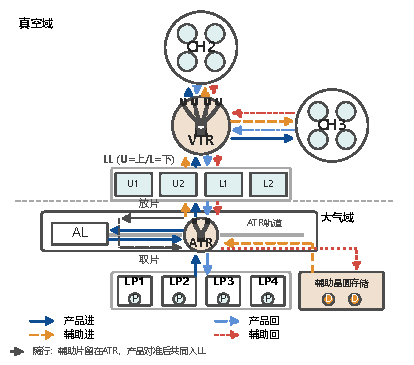
\includegraphics[width=\linewidth]{fig_single_source_pjob_cn}
\caption{单源旋转腔组合设备的拓扑与晶圆路线。}
\label{fig:single-source-cn}
\end{figure}

\section{晶圆、PW对与腔室周期的匹配关系}
\label{sec:model-assignment-cn}

$4\times1$模式在相邻加工周期之间更换全部4片晶圆，$2\times2$模式每次更换2片晶圆并保留另2片继续处理。因此，
将晶圆组织为PW对，再将PW对分配到兼容腔室及其加工周期。每个PW对包含两片晶圆，对内位置$r\in\{0,1\}$是配对索引，
实际承片位置和腔内占位由后续资源与周期变量确定。生产与清洁共用候选加工周期，具体生产次数和清洁规则见第~\ref{sec:model-process-cn}节。

\noindent\textbf{晶圆配对与腔室选择：}
一个PW对可由两片产品、一片产品与一片辅助晶圆，或两片辅助晶圆组成。所有产品均须安排加工，且每个启用对内位置恰好安排一片晶圆。因此，有
\begin{equation}
\begin{aligned}
\sum_{p,r}x_{j\ell pr}&=N_{j\ell},\\
\beta_{pr}=\sum_{j,\ell}x_{j\ell pr},\qquad
\beta_{pr}+d_{pr}&=v_p.
\end{aligned}
\label{eq:joint-membership-cn}
\end{equation}
式~\eqref{eq:joint-membership-cn}满足各任务的LP库存与对内位置唯一占用要求；各位置保留完整加工路线，实际产品身份在求解后恢复。
动作下标$o$可写成$(i,a)$、$(p,a)$或$(c,q,a)$，分别定位晶圆路线、PW对或腔室周期中的动作，$a$为动作标签；起止时刻统一记为$s_o,e_o$。

\noindent\textbf{批次内非递减顺序出片：}
按给定的非递减出片规则，同一批次任务在较小编号LP中的产品取片不得晚于下一非空LP中的产品。
$h_j(\ell)=\min\{\ell'>\ell:N_{j\ell'}>0\}$表示任务$j$在LP $\ell$之后的首个非空LP编号，集合为空时不
建立对应变量。对每个对内位置$(p,r)$，以下$o=((p,r),\mathrm{pick})$定位其LP取片动作。相邻非空LP之间满足：
\begin{equation}
\begin{aligned}
0\le\theta_{j\ell}&\le B,\\
s_o&\le\theta_{j\ell}+M(1-x_{j\ell pr}),\\
s_o&\ge\theta_{j\ell}-M(1-x_{j,h_j(\ell),pr}).
\end{aligned}
\label{eq:pjob-release-boundary-cn}
\end{equation}
式~\eqref{eq:pjob-release-boundary-cn}约束跨LP取片顺序，同一任务、同一LP的产品按取片时刻恢复实际编号，从而满足批次内非递减出片。同一PW对中来自同一LP的产品允许同步取片，但仍须满足式~\eqref{eq:stage-link-cn}及机械手容量约束；其他取片按ATR互斥与换位条件执行。不同Pjob可交错取片，并在工艺相容时组对。

同一PW对中的两片晶圆应采用相容的工艺模式，并进入共同允许的腔室。令$\mathcal C(m)\subseteq\mathcal C$为可执行加工类型$m$的腔室集合，模式与腔室选择满足：
\begin{equation}
\begin{aligned}
\sum_m\mu_{pm}&=v_p,\qquad \sum_c z_{pc}=v_p,\\
x_{j\ell pr}&\le\mu_{p,m_j},\qquad
x_{j\ell pr}\le\sum_{c\in\mathcal C_j}z_{pc},\\
z_{pc}+\mu_{pm}&\le1\qquad(c\notin\mathcal C(m)).
\end{aligned}
\label{eq:joint-chamber-cn}
\end{equation}
同模式的不同任务可组对，所选腔室须属于对内产品允许腔室集合的交集；允许访问两腔的任务可将不同PW对分配至不同腔室。

产品状态、链式模式标记与清洁类型之间满足：
\begin{equation}
\begin{aligned}
F_p&\le\sum_r\beta_{pr}\le2F_p,\qquad F_p+\mu_{p,\mathrm{cl}}\le1,\\
F_p^\psi&\le F_p,\quad F_p^\psi\le\mu_{p\psi},\quad
F_p^\psi\ge F_p+\mu_{p\psi}-1.
\end{aligned}
\label{eq:pair-type-cn}
\end{equation}
位置$(p,r)$的产品来源及回片LP直接由$\sum_jx_{j\ell pr}$确定，辅助来源位置分别由$(1-\sigma)d_{pr}$与$\sigma d_{pr}$确定。

\noindent\textbf{候选容量上界：}
为联合配对与周期决策预留足够的候选编号，采用以下保守容量上界：
\begin{equation}
\begin{gathered}
T=N_{\zeta}+2N_{\psi},\qquad J_{\max}=T,\\
P_{\max}=N+T+2J_{\max},\qquad Q_{\max}=T+J_{\max}.
\end{gathered}
\label{eq:candidate-bounds-cn}
\end{equation}
每个生产周期至少含一片产品，故生产周期数不超过总处理次数$T$；每次清洁前至少有一个生产周期，故清洁次数不超过$T$。含产品对、生产补位对和清洁对分别至多为$N$、$T$和$2J_{\max}$个，得到式~\eqref{eq:candidate-bounds-cn}的容量上界，保留所有合法的提前清洁选择。PW对按一次装入至卸出的占位任务编号，与可复用实体辅助片的库存分别计量。

\noindent\textbf{PW对与加工周期匹配：}
腔室执行生产或清洁时均应保持四工位满片，即每个周期恰好容纳两个PW对。$U_{cq}$是二元辅助变量，表示腔室$c$的周期$q$是否启用。所选
PW对的腔室与加工类型须与周期一致，因此，有：
\begin{equation}
\begin{aligned}
\sum_mK_{cqm}&=U_{cq}, &\sum_pX_{pcq}&=2U_{cq},\\
X_{pcq}&\le z_{pc}, &X_{pcq}+\mu_{pm}&\le1+K_{cqm},\\
\sum_pX^P_{pcq}&\ge K_{cq\zeta}+K_{cq\psi}, &U_{c,q+1}&\le U_{cq},\\
\sum_{c,q}U_{cq}&\le Q_{\max}, &\sum_{c,q}K_{cq,\mathrm{cl}}&\le J_{\max}.
\end{aligned}
\label{eq:cycle-capacity-cn}
\end{equation}
含产品PW对是否参与加工周期，由以下线性约束确定：
\begin{equation}
X^P_{pcq}\le X_{pcq},\quad X^P_{pcq}\le F_p,\quad
X^P_{pcq}\ge X_{pcq}+F_p-1.
\label{eq:cycle-products-cn}
\end{equation}
式~\eqref{eq:cycle-capacity-cn}保证满片加工、PW对与周期相容及候选容量限制；式~\eqref{eq:cycle-products-cn}保证只有含产品对的
占位计入生产要求。由此，生产周期至少含一个产品对，清洁周期只含辅助对。周期按编号连续启用，但不同加工模式的先后次序仍由模型确定。

\section{动作时间与先后逻辑}
\label{sec:model-time-cn}

晶圆操作须满足路线先后关系，成对搬运还须满足两片晶圆的取放同步条件；共享资源的服务次序由第~\ref{sec:model-resource-cn}节的约束确定。

\noindent\textbf{动作启用与持续时间：}
动作启用状态由所选晶圆路线、腔室周期及搬运方式共同确定。已启用动作的持续时间为输入参数，未启用动作的起止时刻均置零；其中LP取片时长满足$d_o>0$。因此，有：
\begin{equation}
0\le s_o\le B b_o,\qquad
0\le e_o\le B b_o,\qquad
e_o=s_o+d_ob_o.
\label{eq:operation-time-cn}
\end{equation}
式~\eqref{eq:operation-time-cn}保证取放、对准、压力转换、旋转及加工动作按给定时长执行，等待只能发生在动作之间。产品对准动作由$\beta_{pr}$启用，源端、ATR与装载锁动作由$\beta_{pr}+(1-\sigma)d_{pr}$启用，VTR供回动作由$v_p$启用。

\noindent\textbf{路径对应的动作先后关系：}
令$\mathcal A$为腔内共同动作链与各晶圆供回路线的已启用先后弧集合；供回路线按来源$\chi_{i\varsigma}$及成对搬运、单源随行入片选择启用，$\varsigma\in\mathcal S$。对弧$(o,o')\in\mathcal A$，后继须在前驱完成并经过必要间隔后开始，且后继启用时前驱也须启用：
\begin{equation}
b_{o'}\le b_o,\qquad
s_{o'}\ge e_o+\delta_{oo'}-M(2-b_o-b_{o'}).
\label{eq:precedence-cn}
\end{equation}
式~\eqref{eq:precedence-cn}连接所选路线的装载、加工与卸载事件。时刻均在$[0,B]$内，$M$覆盖时域与必要间隔，使未启用条件下的时序约束充分放松。

\noindent\textbf{单片、批次与成对搬运动作的同步：}
对需同步的动作$o,o'$，令$x$引用相应LP所属、周期占位或搬运选择的既有二元变量，统一要求：
\begin{equation}
\begin{aligned}
-M(1-x)&\le s_o-s_{o'}\le M(1-x),\\
-M(1-x)&\le e_o-e_{o'}\le M(1-x).
\end{aligned}
\label{eq:stage-link-cn}
\end{equation}
式~\eqref{eq:stage-link-cn}使单片动作与其所属批次的对应动作同时开始、同时结束；成对搬运取$x=\gamma_{pa}$、$o=((p,0),a)$及$o'=((p,1),a)$。同步时机械手执行一次共同动作，与其他动作保持互斥，两片晶圆仍分别占用承片位置；未同步时按式~\eqref{eq:resource-order-cn}分别排序。

\noindent\textbf{单源产品--辅助对的入片逻辑：}
对于单源产品--辅助对，$i_{\rm P},i_{\rm D}$是路线任务索引，分别表示该对中产品与辅助晶圆的路线，下标$\mathrm P,\mathrm D$是晶圆类型标签。
$\gamma^{\rm early}_p,\gamma^{\rm late}_p,\gamma_{p,\mathrm{in}}$是二元决策变量，分别表示是否选择辅助晶圆先行入锁、产品放至AL后再取辅助
晶圆、辅助晶圆随产品入锁。动作标签$\mathrm{ALput,ALpick,LLput}$分别表示放至AL、从AL取回和放入上装载锁。三种路线择一：
\begin{equation}
\begin{gathered}
\gamma^{\rm early}_p+\gamma^{\rm late}_p+\gamma_{p,\mathrm{in}}=1,\\
\gamma^{\rm early}_p=1\Rightarrow e_{(i_{\rm D},\mathrm{LLput})}\le s_{(i_{\rm P},\mathrm{ALput})},\\
\gamma^{\rm late}_p=1\Rightarrow s_{(i_{\rm D},\mathrm{pick})}\ge e_{(i_{\rm P},\mathrm{ALput})},\\
\gamma_{p,\mathrm{in}}=1\ \Longrightarrow
\begin{cases}
e_{(i_{\rm D},\mathrm{pick})}\le s_{(i_{\rm P},\mathrm{ALput})},\\
s_{(i_{\rm D},\mathrm{LLput})}=s_{(i_{\rm P},\mathrm{LLput})},\\
e_{(i_{\rm D},\mathrm{LLput})}=e_{(i_{\rm P},\mathrm{LLput})},\\
s_{(i_{\rm P},\mathrm{LLput})}\ge e_{(i_{\rm P},\mathrm{ALpick})}.
\end{cases}\end{gathered}
\label{eq:single-source-accompany-cn}
\end{equation}
该条件表示辅助晶圆在产品放至AL前已由ATR承载，并与完成对准的产品同时放入上装载锁。辅助晶圆从源端取片至入锁结束持续占用一个ATR承片位置；产品占
用AL期间不占用ATR承片位置，取回后恢复占用。若辅助晶圆单独供给，则直接连接其源端取片与入锁事件。

\section{两种工艺模式与清洁处理}
\label{sec:model-process-cn}

在第~\ref{sec:model-assignment-cn}节的PW对与周期指派关系基础上，进一步约束加工次数、相邻周期的占位连续性、旋转装卸次序及清洁边界；时刻变量沿用第~\ref{sec:model-time-cn}节的定义。

\noindent\textbf{生产模式与连续占位：}
图~\ref{fig:chain-zh}和图~\ref{fig:parallel-zh}给出两种工艺模式的事件顺序，其加工次数与连续性由周期占位约束描述。

\begin{figure}[t]
\centering
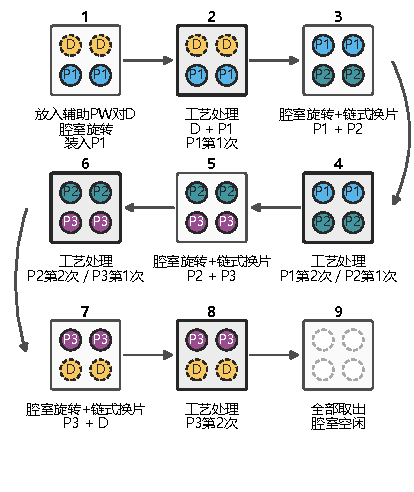
\includegraphics[width=0.93\linewidth]{fig_chain_cn_nature}
\caption{$2\times2$链式生产的事件顺序，D表示辅助PW对。}
\label{fig:chain-zh}
\end{figure}

\begin{figure}[t]
\centering
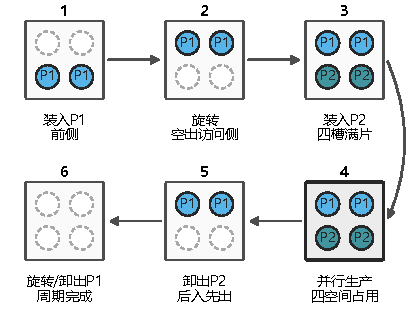
\includegraphics[width=\linewidth]{fig_parallel_cn_nature}
\caption{$4\times1$并行生产的事件顺序。}
\label{fig:parallel-zh}
\end{figure}

$A_{pcq},Z_{pcq}$是二元辅助变量，分别表示对$p$是否在腔室$c$的周期$q$首次、末次参加处理；$A^\psi_{pcq},Z^\psi_{pcq}$是二元辅助变量，分别表示上
述首次、末次参加处理的对是否为$2\times2$含产品对。取边界$X_{pc0}=X_{pc,Q_{\max}+1}=A_{pc,Q_{\max}+1}=0$，且$A_{pc1}=X_{pc1}$直接代入，有：
\begin{equation}
\begin{aligned}
A_{pcq}&\ge X_{pcq}-X_{pc,q-1}, &A_{pcq}&\le X_{pcq},\\
A_{pcq}&\le1-X_{pc,q-1},\\
Z_{pcq}&=X_{pcq}-X_{pc,q+1}+A_{pc,q+1},\\
\sum_{c,q}X_{pcq}&=v_p+F_p^{\psi}, &\sum_{c,q}A_{pcq}&=v_p,\\
A^{\psi}_{pcq}&=X_{pcq}-Z_{pcq}, &Z^{\psi}_{pcq}&=X_{pcq}-A_{pcq},\\
\sum_pA^{\psi}_{pcq}&\le1, &\sum_pZ^{\psi}_{pcq}&\le1.
\end{aligned}
\label{eq:cycle-exposures-cn}
\end{equation}
式~\eqref{eq:cycle-exposures-cn}使每个启用PW对只进入腔室一次，并连续参加一个或两个周期。前三条不等式给出$A_{pcq}=X_{pcq}(1-X_{pc,q-1})$，结合末
次参加标记可得$\sum_{c,q}Z_{pcq}=\sum_{c,q}A_{pcq}=v_p$。含产品的$4\times1$对参加一次处理，含产品的$2\times2$对在同腔参加相邻两次处理，纯辅助补
位对与清洁对均只参加一个周期。

\noindent\textbf{加工时长与周期先后关系：}
一个加工周期只有在前一周期结束后才能开始，持续时间由所选加工类型确定，周期结束时刻为$S_{cq}+\sum_m d_mK_{cqm}$，因此，有
\begin{equation}
\begin{aligned}
S_{cq}&\ge0,\\
S_{cq}+\sum_m d_mK_{cqm}&\le B U_{cq},\\
S_{cq}&\ge S_{c,q-1}+\sum_m d_mK_{c,q-1,m}\\
&\quad-M(1-U_{cq})\qquad(q>1).
\end{aligned}
\label{eq:cycle-time-cn}
\end{equation}
该约束固定各类加工周期的持续时间，等待仅发生在动作之间；装卸与旋转的持续时间由相应事件单独计入。

\noindent\textbf{前后侧占位与旋转装卸：}
机械手只能访问腔室前侧，故新装入的PW对位于前侧，保留自上一周期的PW对经旋转转至后侧。$\kappa_{cq},\upsilon_{cq}$是二元辅助变量，分别表示周期$q$是否保
留来自$q-1$的一个PW对、周期$q$结束后是否两个PW对全部退出。根据相邻周期的占位关系，有
\begin{equation}
\begin{aligned}
\kappa_{cq}&=\sum_p(X_{pcq}-A_{pcq}),\\
\upsilon_{cq}&=U_{cq}-\sum_p(X_{pcq}-Z_{pcq}),\\
f_{pcq}&\le A_{pcq},\qquad\sum_pf_{pcq}=U_{cq},\\
f_{pc,q-1}&\ge X_{pcq}-A_{pcq}\quad(q>1),\\
f_{pcq}&\ge F_p+K_{cq\psi}+X_{pcq}-2-\kappa_{cq}.
\end{aligned}
\label{eq:cycle-side-cn}
\end{equation}
动作$(p,\mathrm{load})$与$(p,\mathrm{unload})$分别是PW对$p$的装入与卸出；$(c,q,\mathrm{rot-})$与$(c,q,\mathrm{rot+})$分别是该周期前、后的半周旋转，
由$U_{cq}$与$\upsilon_{cq}$启用，各持续$r_c$，装入与旋转的时序约束为
\begin{equation}
\begin{aligned}
X_{pcq}=1\ \Rightarrow\quad
&S_{cq}\ge e_{(p,\mathrm{load})},\\
&s_{(p,\mathrm{unload})}\ge S_{cq}+\sum_m d_mK_{cqm};\\
A_{pcq}=1,\ f_{pcq}=0\ \Rightarrow\quad
&e_{(p,\mathrm{load})}\le s_{(c,q,\mathrm{rot-})};\\
A_{pcq}=1,\ f_{pcq}=1\ \Rightarrow\quad
&s_{(p,\mathrm{load})}\ge e_{(c,q,\mathrm{rot-})},\\
&S_{cq}=e_{(p,\mathrm{load})};\\
\kappa_{cq}=1\ \Rightarrow\quad
&s_{(c,q,\mathrm{rot-})}\ge S_{c,q-1}\\
&\qquad+\sum_m d_mK_{c,q-1,m}.
\end{aligned}
\label{eq:cycle-load-cn}
\end{equation}
全部退出时，周期后旋转在加工结束后开始。最后一次加工后的卸片关系为
\begin{equation}
\begin{aligned}
Z_{pcq}=1,\ f_{pcq}=1\quad
&\Rightarrow e_{(p,\mathrm{unload})}\le s_{(c,q,\mathrm{rot+})},\\
Z_{pcq}=1,\ f_{pcq}=0,\ \upsilon_{cq}=1\quad
&\Rightarrow s_{(p,\mathrm{unload})}\ge e_{(c,q,\mathrm{rot+})},\\
Z_{pcq}=1,\ f_{pcq}=0,\ \upsilon_{cq}=0\quad
&\Rightarrow s_{(p,\mathrm{unload})}\ge e_{(c,q+1,\mathrm{rot-})}.
\end{aligned}
\label{eq:cycle-unload-cn}
\end{equation}
下一周期新装入的PW对必须等待上一周期所有退出对完成卸载。对$p,p'\in\mathcal P$及$q>1$，有：
\begin{equation}
\begin{aligned}
s_{(p',\mathrm{load})}&\ge e_{(p,\mathrm{unload})}\\
&\quad-M(2-Z_{pc,q-1}-A_{p'cq}).
\end{aligned}
\label{eq:cycle-exchange-cn}
\end{equation}
保留一个对时，式~\eqref{eq:cycle-exchange-cn}仅等待被替换对卸出；全部退出时则等待两对均卸完，并与VTR动作互斥共同约束换片。

\noindent\textbf{清洁触发与清洁动作链：}
用清洁计数器累计自上次清洁以来的生产周期数，完成清洁后计数归零。达到阈值时须执行清洁，未达到阈值时可在合法工艺边界提前清洁；初始清洁与连续清洁均不允许。
取候选尾部$U_{c,Q_{\max}+1}=0$，有：
\begin{equation}
\begin{aligned}
0\le n_{cq}&\le H U_{cq},\qquad n_{c0}=0,\\
K_{cq,\mathrm{cl}}=1&\Rightarrow n_{cq}=0,\\
U_{cq}=1,\ K_{cq,\mathrm{cl}}=0
&\Rightarrow n_{cq}=n_{c,q-1}+1,\quad n_{c,q-1}\le H-1,\\
K_{cq,\mathrm{cl}}=1&\Rightarrow 1\le n_{c,q-1}\le H,\\
n_{cq}&\le H-1+H U_{c,q+1}.
\end{aligned}
\label{eq:clean-counter-cn}
\end{equation}
式~\eqref{eq:clean-counter-cn}在达到阈值时强制清洁，包括最后一个生产段；初始计数为零、清洁前计数至少为1及清洁后归零共同禁止初始清洁和连续清洁。由式~\eqref{eq:cycle-capacity-cn}与式~\eqref{eq:cycle-exposures-cn}，同一链式产品对须连续参加两个生产周期，清洁不能插入其中。

清洁作为$m=\mathrm{cl}$的满片周期，由两个纯辅助PW对占位，与生产共用式~\eqref{eq:cycle-load-cn}--\eqref{eq:cycle-exchange-cn}的装卸与旋转规则：两侧装入四片辅助晶圆后清洁，再依次卸出。相邻周期的换片约束要求清洁前卸完原有晶圆，清洁后卸完辅助片，再装入下一周期的晶圆；VTR互斥及辅助片借还约束共同确定搬运与复用时刻。

\section{辅助晶圆复用与机械手、模块资源}
\label{sec:model-resource-cn}

实体资源可用性通过辅助晶圆身份指派、机械手承片位置与模块槽位分配、占用互斥及驻留上限约束共同保证。

\noindent\textbf{辅助晶圆与循环复用：}
两腔共享辅助晶圆库存，一片辅助晶圆在归还之前不能再次借出。因此，每项有效借用需求应选定一片实体晶圆，同一PW对的两个位置应使用不同晶圆，有
\begin{equation}
\sum_{\tau\in\mathcal D}g_{pr\tau}=d_{pr},\qquad
\sum_{r=0}^{1}g_{pr\tau}\le1.
\label{eq:dummy-assign-cn}
\end{equation}
式~\eqref{eq:dummy-assign-cn}保证每项辅助需求恰好分配一片晶圆。借用区间按共享资源约束排序，使同一晶圆只能在完成归还后再次使用。该条件同样适用于跨
腔借用，允许两腔使用不同辅助晶圆并行生产。

\noindent\textbf{机械手与模块容量：}
资源排序区分执行机构的动作互斥与承片位置的容量限制。ATR、VTR、AL及各旋转腔的执行机构作为独占动作资源；机械手承片位置、装载锁槽位和辅助晶圆身份分别分配物理单元，容量采用表~\ref{tab:symbol-cn-a}的配置。腔内占位已由式~\eqref{eq:cycle-capacity-cn}约束。

资源分配以单个占用区间为单位：一次单片承片位置占用、一次辅助晶圆借用或一次执行机构互斥占用均选择一个允许单元。对$\mathcal O^{\rm occ}$中的占用区间，
$\Gamma_o$是允许物理单元的集合，按晶圆类型及各物理单元允许执行的动作确定；若所选晶圆类型不同，则启用该类型对应的资源选择约束。占用分配满足：
\begin{equation}
\sum_{u\in\Gamma_o}h_{ou}=b_o,\qquad 0\le s_o,e_o\le B.
\label{eq:slot-select-cn}
\end{equation}
式~\eqref{eq:slot-select-cn}保证启用占用恰好选择一个允许单元；占用结束时刻计入复位尾部后仍须满足统一时间界。两片晶圆成对搬运时，各自保留承片位置占
用，动作同步由式~\eqref{eq:stage-link-cn}协调。同一单元的占用区间不重叠，由式~\eqref{eq:resource-order-cn}保证。当$\Gamma_o$仅含一个单元时，$h_{ou}=b_o$可直接代入。

装载锁槽位占用从放片开始，持续到取片完成并加上复位时间，复位只限制该槽位的再次使用，可与取片后机械手的继续运输重叠。

$D_1,D_2,C_1,C_2$是物理手的固定编号，依次表示VTR的两只脏手和两只洁净手。未完成工艺处理的产品晶圆由脏手搬运，$\Gamma_o=\{D_1,D_2\}$；
完成全部工艺处理的产品晶圆由洁净手搬运，$\Gamma_o=\{C_1,C_2\}$。辅助晶圆的输入与返回均允许$\Gamma_o=\{D_1,D_2,C_1,C_2\}$。每项承
片任务从取片动作开始持续至放片动作完成，式~\eqref{eq:slot-select-cn}选择的物理手在此区间内保持不变。相同手上的占用按式~\eqref{eq:resource-order-cn}
互斥，其承片区间的换位间隔取零。脏手与洁净手各自最多承载两片，辅助晶圆同时竞争这两类空闲承片位置，每项辅助晶圆承片任务均须指派至满足占用互斥条件的具体物理手。

\noindent\textbf{资源互斥与地点相关换位：}
共享资源的先后关系分为给定技术次序和待定服务次序。路线先后弧按工艺执行，其余冲突动作通过资源次序变量协调。

若两个动作占用选择同一资源单元，则其中一个必须在另一个结束后开始，并满足换位或复位间隔。因此，有：
\begin{equation}
\begin{aligned}
s_{o'}&\ge e_o+\delta^\rho_{oo'}-M(1-y^\rho_{oo'})
-M(1-h_{ou})-M(1-h_{o'u}),\\
s_o&\ge e_{o'}+\delta^\rho_{o'o}-My^\rho_{oo'}
-M(1-h_{ou})-M(1-h_{o'u}).
\end{aligned}
\label{eq:resource-order-cn}
\end{equation}
式~\eqref{eq:resource-order-cn}保证选用同一物理单元的占用区间不重叠；选用不同单元时，该对互斥条件不限制其并行。该约束分别用于机械手
动作、物理手、模块槽位、腔室执行机构和实体辅助晶圆。

换位时间按地点对给定。对于腔室由$z_{pc}$决定的动作，按候选腔室组合启用相应移动时间间隔，而不预先固定其地点。$p',c'$分别是另一PW对及
其腔室的索引；$\delta^{\rm VTR}_{cc'}$是非负实数常量，表示VTR从腔室$c$移至$c'$的时长。例如，两动作分别服务于对$p,p'$且均启用时，有：
\begin{equation}
\begin{aligned}
z_{pc}=z_{p'c'}=1,\ y^{\rm VTR}_{oo'}=1
\ \Rightarrow\ s_{o'}\ge e_o+\delta^{\rm VTR}_{cc'}.
\end{aligned}
\label{eq:location-travel-cn}
\end{equation}
对固定地点的动作，直接使用式~\eqref{eq:resource-order-cn}。产品的来源与回片LP均由$\sum_jx_{j\ell pr}$确定，移动间隔同样按地点组合条
件启用，且回到所选原LP。

\noindent\textbf{驻留限制与死锁预防：}
对启用的晶圆路线任务，$\operatorname{in}(i,\rho)$和$\operatorname{out}(i,\rho)$分别表示将晶圆$i$放入模块$\rho$、从该模块取出的动
作索引。对于AL和装载锁，直接限制这两个端点之间的时长；对于工艺腔，先扣除该晶圆所在PW对实际参加的必要工艺处理时长，再限制剩余的非加工
驻留时间。必要工艺处理包括生产处理和清洁处理，不包括等待、旋转及其他取放动作；扣除时长按式~\eqref{eq:cycle-exposures-cn}确定的参与次数计算。对启用路线$i=(p,r)$，有：
\begin{equation}
\begin{aligned}
0\le\;&s_{\operatorname{out}(i,\rho)}-e_{\operatorname{in}(i,\rho)}
\le\overline R_{i\rho},\quad \rho\notin\mathcal C;\\
0\le\;&s_{(p,\mathrm{unload})}-e_{(p,\mathrm{load})}
-d_\zeta\mu_{p\zeta}\\
&-d_\psi(\mu_{p\psi}+F_p^\psi)
-d_{\mathrm{cl}}\mu_{p,\mathrm{cl}}\le\overline R_{i\rho},
\quad\rho\in\mathcal C.
\end{aligned}
\label{eq:residence-cn}
\end{equation}
式~\eqref{eq:residence-cn}中的第二组约束用于路线实际访问的工艺腔。占用结束时刻连同复位尾部均不超过$B$。

上述操作先后约束~\eqref{eq:precedence-cn}与资源排序约束~\eqref{eq:resource-order-cn}共同构成本模型的死锁避免机制。对任一候选排程，
以已激活操作为节点，以操作先后关系及求解器确定的共享资源次序为有向弧；若机械手、装载锁、旋转腔或辅助晶圆之间出现循环等待，则
该操作--资源图中必然出现有向环。对于实际资源占用操作，沿环累加相应时间约束会产生正的持续时间或切换时间增量，从而要求某一操作的开始时
刻严格晚于自身，违反时间可行性。因此，在给定设备参数下，满足上述时间约束的排程排除了已建模操作与资源之间的循环等待。

\section{完工时间优先的两阶段优化}
\label{sec:model-objective-cn}

$\mathcal F$是由前述全部约束确定的联合可行域；$\xi$是变量向量，表示模型全部保留变量的整体赋值。第一阶段优化产品回片完工时间，第二阶
段在保留第一阶段完工时间上界与主要离散结构的条件下优化等待与生产节拍。

第一阶段联合调整产品配对、腔室分配、加工周期与资源使用次序，以缩短产品完工时间；第二阶段固定其中的主要离散决策，继续调整动作时刻和取放同步选择，以改善等待与节拍。第二阶段以第一阶段的产品完工时间及给定容差限制完工上界。

\noindent\textbf{第一阶段：最小化产品回片完工时间：}
对每个位置$(p,r)$，以下$o=((p,r),\mathrm{return})$定位其返回原LP的动作，$\mathrm{return}$是回片动作标签。只对产品晶圆形成主目标下界：
\begin{equation}
\begin{gathered}
C_{\max}\ge e_o-M(1-\beta_{pr})\quad(p,r),\\
\min_{\xi\in\mathcal F}C_{\max}.
\end{gathered}
\label{eq:primary-objective-cn}
\end{equation}
式~\eqref{eq:primary-objective-cn}表示最大完工时间按最后一片产品晶圆完成完整端到端路线并返回LP的时刻计算。若清洁位于两个生产段之间，
其资源占用与时序约束通过后续产品回片时间影响$C_{\max}$；若最后一次清洁之后不再有产品工艺处理，则该末端清洁仍保留在设备动作序列
中，其完成时刻不直接作为$C_{\max}$的下界。末端清洁仍可能经共享VTR与其他腔室的产品回片竞争资源，因此其间接影响须由完整排程判定。产品产
出率按$\mathrm{WPH}=3600N/C_{\max}$统计，单位为片/小时；该值以批次开始至最后一片产品回到LP为统计区间，表示有限批次的等效产出率。

\noindent\textbf{第二阶段：限定优化范围并精修时序：}
以第一阶段当前最好可行赋值$\widehat\xi$及其产品完工时间$\widehat C$为参考。$\mathcal D_{\rm fix}$包含配对、分腔、周期占位、辅助身份、手分配、随行入片及资源次序的变量分量索引，排除可继续调整的取放同步选择。第二阶段在原可行域上增加：

\begin{equation}
\begin{gathered}
\xi_d=\widehat\xi_d\quad(d\in\mathcal D_{\rm fix}),\qquad
C_{\max}\le\widehat C+\varepsilon_C.
\end{gathered}
\label{eq:secondary-domain-cn}
\end{equation}

式~\eqref{eq:secondary-domain-cn}固定分量$d$的赋值$\xi_d=\widehat\xi_d$，同地点取放动作的同步选择与连续时刻继续参与优化。

$\mathcal W$是供回片路线等待项的索引集合；$\omega_\alpha$表示等待项$\alpha$对应的时刻差表达式，即后继动作开始时刻减去前驱动作结束时
刻，再扣除必要操作或移动时长。所有晶圆均计入VTR源端取片结束至对装片开始、对卸片结束至VTR目的端放片开始的间隔，并扣除必要移动时间。经过
大气侧的晶圆还计入相邻动作之间的间隔，分别扣除移动、对准、抽气或放气时长；绕过AL的辅助片以源端取片至上锁放片代替前三项。各间隔均按前一
动作结束至后一动作开始计算。腔内加工结束至卸片开始的间隔由周期、驻留和资源约束管理，供回路线等待与腔内驻留分别统计。

总路线等待按$\sum_{\alpha\in\mathcal W}\omega_\alpha$计算，实验统计简记为$L_{\rm sum}$。产品片与辅助片均纳入评价，并行发生的不同晶
圆等待分别计入。最大单项等待满足：
\begin{equation}
L_{\max}\ge\omega_\alpha\ge0,\qquad \alpha\in\mathcal W.
\label{eq:secondary-wait-cn}
\end{equation}

$\mathcal I_{\rm rhythm}$是节拍评价中心的索引集合，包含同一腔室、同一$2\times2$链内连续三个生产周期的中心$(c,q)$；相邻两处边界均保
留一个对，即$\kappa_{cq}=\kappa_{c,q+1}=1$，不跨清洁或链边界计算。第二阶段固定周期结构后，该集合随之确定。后一个开始间隔减去前一个间
隔为$S_{c,q+1}-2S_{cq}+S_{c,q-1}$，其绝对值上界满足：

\begin{equation}
\begin{aligned}
v_{cq}&\ge S_{c,q+1}-2S_{cq}+S_{c,q-1},\\
v_{cq}&\ge-S_{c,q+1}+2S_{cq}-S_{c,q-1}
\quad((c,q)\in\mathcal I_{\rm rhythm}).
\end{aligned}
\label{eq:secondary-rhythm-cn}
\end{equation}

将上述指标按给定权重组合，第二阶段目标为：
\begin{equation}
\begin{aligned}
\min\ \ &\lambda_1\sum_{\alpha\in\mathcal W}\omega_\alpha+\lambda_2L_{\max}\\
&+\lambda_3\sum_{(c,q)\in\mathcal I_{\rm rhythm}}v_{cq}.
\end{aligned}
\label{eq:secondary-objective-cn}
\end{equation}

式~\eqref{eq:secondary-objective-cn}组合总等待、最大单项等待与节拍变化三项指标。当对应权重严格为正且第二阶段达到最优时，$L_{\max}=\max_\alpha\omega_\alpha$、$v_{cq}=|S_{c,q+1}-2S_{cq}+S_{c,q-1}|$。实验指标统一由实际事件时刻计算；连续三个生产周期等间隔开始时，节拍变化为零。驻留上限仍作为硬约束执行。第~\ref{sec:third-innovation}~节在同一配置D可行域上同时最小化产品完工时间与上述综合指标，考察放宽交期所能换取的等待与节拍改善。


\FloatBarrier
\section{模型完整线性化与表示等价性}
\subsection{固定候选索引、激活条件与大常数有效性}
\vspace*{3cm}
\subsection{库存解码与显式晶圆表示的对应证明}
\vspace*{3cm}
